\section{Commutativity rewrites}

\begin{definition}
For any node variables $a,b \in \Upsilon$: 
\begin{enumerate}
\item[-] the first C rewrite is: $\displaystyle \left(a b \right)^{e} x \, \longleftrightarrow \, \left(b a  \right)^{e} x$
\item[-] the second C rewrite is: $\displaystyle \left(\bar{a} \bar{b} \right)^{e} x \, \longleftrightarrow \, \left(\bar{b} \bar{a}  \right)^{e} x$
\item[-] the third C rewrite is: $\displaystyle \left(\bar{a} b \right)^{e} x \, \longleftrightarrow \, \left(b \bar{a}  \right)^{e} x$
\end{enumerate}
\centerline{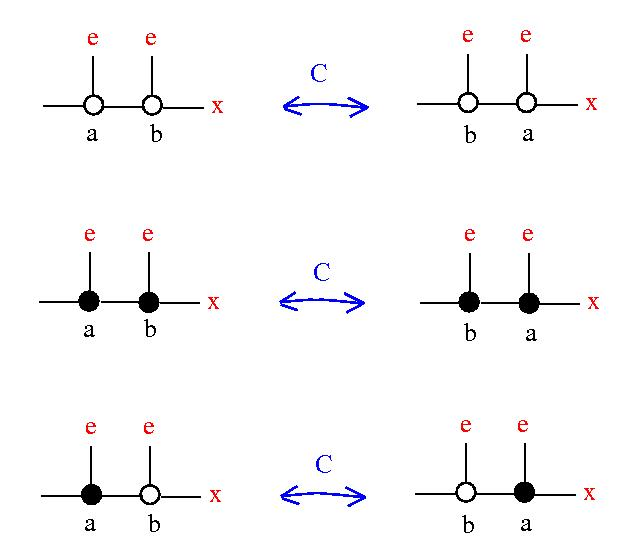
\includegraphics[width=80mm]{jpg/accept_3.jpg}}  
\label{c}
\end{definition}


\begin{proposition}
In the presence of the third C rewrite, the R2 rewrites are equivalent with: for any $a \in \Upsilon$ and any binary term $b$ 
\begin{equation}
 a - (a - b)^{e} x \, \longleftrightarrow \, b^{e} x 
\label{aab}
\end{equation}
\end{proposition}

\paragraph{Proof.} The third C rewrite can be used to show that the two R2 rewrites are equivalent. Use then Proposition \ref{pr2} to get that the two R2 rewrites are equivalent with 
(\ref{2r2}), (\ref{1r2}). Use the Figure \ref{a-(a-b)-fig} to deduce (\ref{aab}). Conversely, (\ref{aab}) applied for $b = 0$ gives (\ref{2r2}) and for $b = 1$ gives (\ref{1r2}). 


\vspace{.5cm} 



There is no meaning for $a-b$ when $a, b \in Y$, in the realm of $Y$-irqs. However, looking back to the simple example of a $(0, \infty)$-irq made from a real vector space, we saw that $a-b$ (from Definition 
\ref{ddifprod}) does mean what is expected. On the other side, there are far more examples of irqs where there is no clear correspondent for this "$a-b$" operation. 
